\chapter{Aprendizaje transferible y multi-tarea}%
\label{cha:aprendizaje_transferible_y_multi_tarea}

\lecture{16}{2020-07-08}{Transfer and Multi-Task Learning}

\section{¿Cuál es el problema?}%
\label{sec:_cuál_es_el_problema_}

Para tareas 'simples' como por ejemplo Breakout, los algoritmos vistos hasta ahora funcionan
razonablemente bien. Pero para entornos complejos como por ejemplo \textit{Montezuma's
Revenge} estos algoritmos fallan catastróficamente. Esto es porque este tipo de juegos requiere
un entendimiento de qué significan los \textit{sprites} que salen por pantalla. Por
ejemplo:
\begin{itemize}
    \item La llave: abre puertas
    \item Escaleras: se pueden subir
    \item Calavera: no se sabe lo que hace exactamente, pero se sobreentiende que
        nada bueno.
\end{itemize}
Un conocimiento previo de la estructura del problema puede ayudarnos a resolver tareas
complejas rápidamente.

\subsection{¿Puede RL usar el mismo conocimiento previo que nosotros?}%
\label{sub:_puede_rl_usar_el_mismo_conocimiento_previo_que_nosotros_}

La idea está en que una vez se hayan resuelto otras tareas, es posible que se haya obtenido un
conocimiento útil para resolver otra tarea nueva.

Hay varias formas de guardar el conocimiento:
\begin{itemize}
    \item Función Q: nos dice que estados y acciones son buenos
    \item Política: nos dice que acciones son potencialmente útiles. Algunas acciones puede ser
        que nunca sean útiles.
    \item Modelos: nos dicen las leyes de la física que gobiernan el mundo.
    \item Características/estados ocultos: proveen de una buena representación. Por
        ejemplo, una CNN que detecte elementos de una escena y los codifique. No
        subestimar.
\end{itemize}

\section{Terminología del aprendizaje transferible}%
\label{sec:terminología_del_aprendizaje_transferible}

\begin{itemize}
    \item \textit{Transfer Learning}: usar experiencia de una serie de tareas para un
        aprendizaje más rápido y mejor en otra tarea nueva. En aprendizaje por refuerzo, la
        tarea es el MDP.
    \item \textit{Shot}: número de intentos en el entorno objetivo.
        \begin{itemize}
            \item \textit{0-shot}: simplemente se corre la política entrenada en el
                dominio de la fuente. La política es muy generalizable. Normalmente se
                requieren ciertas asunciones.
            \item \textit{1-shot}: el algoritmo sólo necesita aprender a partir de un
                ejemplo.
            \item \textit{few-shot}: necesita realizar unos pocos episodios para aprender.
        \end{itemize}
\end{itemize}

\section{¿Cómo se pueden plantear los problemas de aprendizaje por transferencia?}%
\label{sec:_cómo_se_pueden_plantear_los_problemas_de_aprendizaje_por_transferencia_}

Hay varias formas de plantearlo, cada una de ellas forma algoritmos diferentes:
\begin{itemize}
    \item \textit{Forward transfer}: entrenar en una tarea, transferir a otra tarea.
    \item \textit{Multi-task transfer}: entrenar en muchas tareas, transferir a otra
        tarea nueva.
    \item \textit{Multi-task meta-learning}: aprender a aprender a partir de muchas tareas
        (próximo tema).
\end{itemize}

\subsection{Forward Transfer}%
\label{sub:forward_transfer}

Se entrena en una tarea y se transfiere a otra tarea. Se puede hacer así burdamente pero lo
mejor es entrenar en una tarea y refinar en otra tarea.

Si se tiene el poder de elegir las tareas fuente, se pueden aleatorizar para aumentar la
generalización.

\subsection{Finetuning}%
\label{sub:finetuning}

Finetuning viene del mundo del aprendizaje supervisado, y su aplicación a RL requiere de ciertos
cambios.

Uno de los problemas más grandes es que al entrenar una política en entornos totalmente
observables, la política óptima siempre será determinista. Los algoritmos que se han visto
hasta ahora van reduciendo la exploración a medida que van convergiendo para aproximarse a esta
política determinista. Por lo que al no haber exploración, pasar esa política a un nuevo
dominio es problemático.

Por lo que normalmente se entrenan políticas algo más estocásticas en los entornos fuente.

\begin{center}
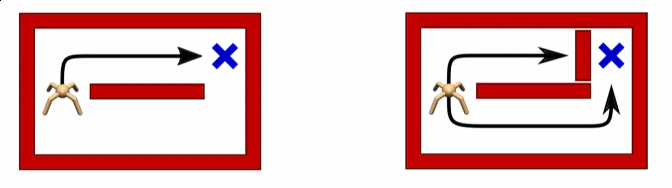
\includegraphics[width=0.5\textwidth]{figures/2020-07-08-151636_672x188_scrot.png}
\end{center}

En el caso que se quiera transferir de la tarea de la izquierda a la de la derecha, es mejor
que al comienzo se entrene una política que llegue al destino por los dos caminos posibles,
aunque el camino largo de menos recompensa. Para esto, se puede utilizar lo que se vio en el
replanteamiento de RL como un problema de inferencia, donde se maximiza tanto la recompensa
como la entropía. Esto hace que en la nueva tarea el agente pueda llegar al destino a partir de
la política original.

En la práctica, una vez que se tenga entrenada la política en el entorno objetivo es
preferible dejar de maximizar la entropía. Para esto se pueden hacer varias cosas:
\begin{itemize}
    \item Entrenar la política con un coeficiente que multiplique a la entropía y vaya
        disminuyendo con el paso del tiempo.
    \item Si se tiene una red neuronal que produce una mezcla de gaussianas en su salida, se
        puede reducir su varianza a 0. Suele funcionar bien pero no está garantizado que
        funcione, ya que el modelo no fue entrenado con varianza nula.
\end{itemize}

Publicaciones importantes sobre \textit{finetuning}:
\begin{itemize}
    \item Finetuning via MaxEnt RL: Haarnoja*, Tang*, et al. (2017). Reinforcement Learning with Deep
    \item Energy-Based Policies.
    \item Finetuning from transferred visual features (via VAE): Higgins et al. DARLA: improving zero-shot
    \item transfer in reinforcement learning. 2017.
    \item Andreas et al. Modular multitask reinforcement learning with policy sketches. 2017.
    \item Florensa et al. Stochastic neural networks for hierarchical reinforcement learning. 2017.
\end{itemize}

\subsubsection{Manipular el dominio fuente}%
\label{ssub:manipular_el_dominio_fuente}

Pueden haber casos en los que los dominios fuente se puedan modificar. Esto ocurre cuando se
diseña una simulación para luego ser aplicada en el mundo real, por ejemplo.

Lo que interesa es tener un entorno fuente en el que el agente aprenda a partir de muchas
muestras muy diversas, para luego aplicarla a otra tarea más específicas con la esperanza de que
el nuevo entorno más especifico se parezca en parte al entorno original.

Por ejemplo, en la publicación \textit{EPOpt: Learning robust neural network policies} se entrena
un agente sobre un robot virtual con masas variantes en sus enlaces. El control robusto
obtenido tiene un precio: para poder funcionar con cualquier tipo de masas, la política no será
la óptima en ninguna de ellas. Esto se acentúa con políticas lineales o poco expresivas, pero con
las redes neuronales este problema se disminuye considerablemente (incluso haciendo que la
diferencia sera casi nula en algunos casos).

Se pueden recoger los parámetros de un robot real para pasarlo a simulación haciendo varias
pruebas con el hardware real y luego entrenar sobre los parámetros físicos obtenidos. Pero
puede resultar ser mejor idea crear un controlador robusto que se adapte a los cambios de esos
parámetros físicos, ya que para los parámetros reales tiene la misma eficiencia que el
controlador específico además de tener un mejor comportamiento con parámetros
distintos.

En otra publicación (\textit{Preparing for the unknown: Learning a Universal Policy with Online
System Identification}), se tiene un diseño más complejo en el que se tiene a una red recurrente
que intenta predecir los parámetros físicos del simulador, para poder meterlos como
entrada a la política, y de esta forma que sepa que acciones tomar.

\begin{center}
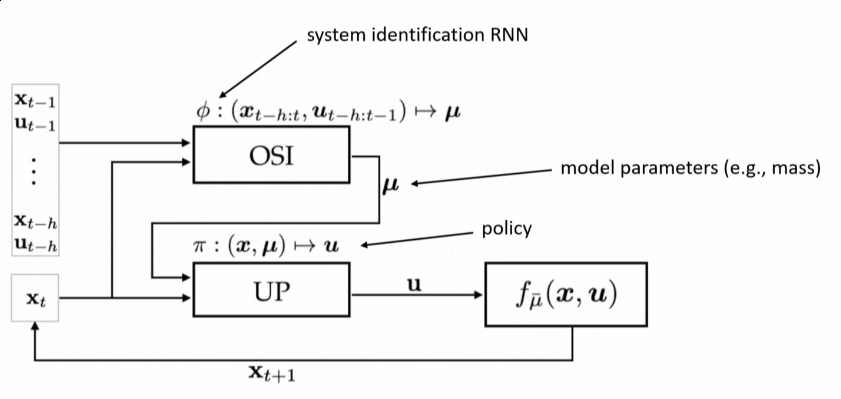
\includegraphics[width=0.8\textwidth]{figures/2020-07-12-185327_841x399_scrot.png}
\end{center}

Estos métodos suponen que no se sabe nada del dominio del objetivo (0-shot), pero en problemas reales si
que se conocen cosas de la tarea que se quiere realizar.

Una de las cosas que se puede hacer es \textit{Adversarial Domain Adaptation}, también
llamado \textit{Domain Confusion}. En el cual se tienen por ejemplo imágenes de simulación con
pocas características e imágenes reales que se corresponden exactamente con las de la
simulación. Se pretende obtener un modelo que saque las mismas características para
dos imágenes correspondientes: una de la simulación y otra de la realidad.

\begin{center}
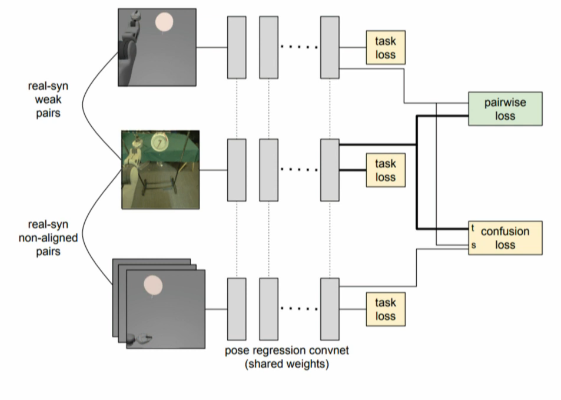
\includegraphics[width=0.5\textwidth]{figures/2020-07-12-190707_561x400_scrot.png}
\end{center}

Hay dos formas de conseguir esto:
\begin{itemize}
    \item Si las dos figuras no son solo análogas sino que también se corresponden con el
        mismo estado exactamente, entonces se pueden regularizar las características para
        que tomen valores similares. Normalmente no se tiene ese conocimiento.
    \item Si no se corresponden pero vienen de de la misma distribución (por ejemplo una política
        aleatoria sobre la simulación y sobre el mundo) se puede utilizar una función de
        pérdida \textit{unpaired distributional alignment} sobre las características. Un
        ejemplo de esta función de pérdida viene prestada de las GANs. Se usa un discriminador
        sobre las características extraídas de las imágenes. Se pretende que la red neuronal
        genere características que hagan que el discriminador no sea capaz de diferenciar su
        procedencia (real o simulación). Esto se conoce como \textit{Domain Adversarial Neural
        Networks}, \textit{Domain Confusion} o \textit{Adversarial Domain Adaptation}.
\end{itemize}

\subsubsection{Resumen del \textit{forward training}}%
\label{ssub:resumen_del_forward training}

\begin{itemize}
    \item Preentrenamiento y finetuning:
        \begin{itemize}
            \item El finetuning estándar aplicado a RL es difícil.
            \item La formulación de la entropía máxima puede ayudar.
        \end{itemize}
    \item Se pude modificar el entorno fuente:
        \begin{itemize}
            \item La aleatorización puede ayudar mucho a crear políticas fuente más diversas.
        \end{itemize}
    \item En el caso que se tengan pocos datos del dominio fuente:
        \begin{itemize}
            \item \textit{Domain adaptation}: hacer que la red neuronal no sea capaz de
                distinguir entre las observaciones de ambos dominios.
            \item O modificar las observaciones en el dominio fuente para que se vean como en
                el dominio objetivo (por ejemplo con una GAN).
        \end{itemize}
\end{itemize}

\subsection{Multi-task transfer}%
\label{sub:multi_task_transfer}

Hasta ahora se usaba un dominio bastante general para poder preentrenar un modelo que
posteriormente lo hiciera bien en una tarea específica. Pero si se quiere entrenar un modelo
para que haga varias tareas, es posible que no haga falta diseñar un entorno fuente tan diverso.

Esto es más cercano a lo que las personas hacemos, que es utilizar lo aprendido en tareas
anteriores para realizar nuevas. Pero es sustancialmente más difícil ya que no todas las tareas
pasadas contribuyen a realizar cualquier tarea nueva, incluso puede ser que dificulte su
aprendizaje.

\subsubsection{RL basado en modelo}%
\label{ssub:rl_basado_en_modelo}

Para este caso la transferencia es fácil de entender. Se busca encontrar que tienen en común
todas las tareas:
\begin{itemize}
    \item Idea 1: las leyes de la física.
        \begin{itemize}
            \item Versión simple: entrenar un modelo en tareas pasadas y usarlo para resolver
                tareas nuevas.
            \item Versión más compleja: se adapta el modelo a la nueva tarea. Es más fácil
                de entrenar que el \textit{finetuning} si las físicas son las mismas pero la
                tarea cambia mucho.
        \end{itemize}
    \item Idea 2: Entrenar todas las políticas de forma separada (MDP diferentes) y después
        unirlas en una única política. Para combinarlos se inicializa las simulaciones con un estado
        inicial y un MDP.
\begin{center}
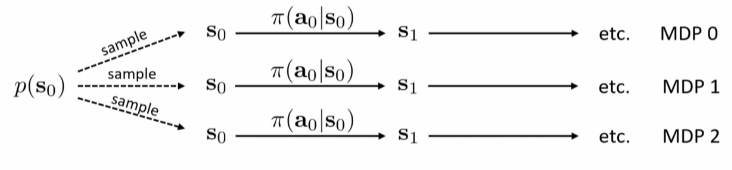
\includegraphics[width=0.8\textwidth]{figures/2020-07-12-195346_732x170_scrot.png}
\end{center}
    Pero esto es una tarea difícil ya que conseguir que un optimizador consiga una
    política que se comporte bien en todos los MDP es una tarea complicada. Por lo que se
    pueden combinar las políticas mediante \textit{Policy Distillation}.
\end{itemize}

\subsubsection{¿Cómo sabe el modelo qué hacer?}%
\label{ssub:_cómo_sabe_el_modelo_qué_hacer_}

En el caso de juegos de Atari, es fácil ya que se puede ver en que juego está simplemente
mirando el estado. Pero hay otros casos como por ejemplo un robot que realice varias tareas en
las que no está tan claro que tarea debe realizar.

Se pueden enumerar las tareas a realizar con un número o representarlas con un vector
\textit{one-hot} y condicionar la política en ese número o vector. (\textit{Contextual Policy:
$\pi_\theta(a|s,\omega)$}). Esto es muy utilizado en robótica y en animación.

\subsubsection{Arquitecturas para multi-task learning}%
\label{ssub:arquitecturas_para_multi_task_learning}

Hasta ahora se ha creado una red neuronal para todas las tareas. Esto no tiene sentido porque
por ejemplo se puede querer una política que controle un coche a partir de la información de
un LiDAR y otro que lo haga a partir de la información de una cámara, o diez robots
intentando hacer tareas distintas. Por lo que interesa crear arquitecturas con componentes
reusables.

En la publicación \textit{Neural Module Networks, Andreas et al.} se hace justo esto. Aunque
trabaja sobre una tarea de aprendizaje supervisado.

\begin{center}
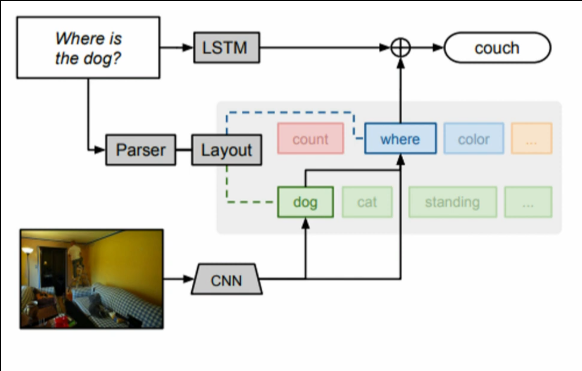
\includegraphics[width=0.6\textwidth]{figures/2020-07-12-200852_582x371_scrot.png}
\end{center}

Su aplicación a RL se explica en \textit{Learning Modular Neural Network Policies, Devin,
Gupta, et al}. En este paper se divide la política en dos partes: la específica del robot y la
específica de la tarea. Por lo que se pueden coger todas las tareas y los robots y distribuirlos
en una matriz. La idea está en que si se entrenan las políticas sobre algunas tareas
compuestas de las combinaciones de la tabla, el robot lo hará bien en combinaciones no vistas o
necesitará muy poco entrenamiento.

En la práctica esto puede ir mal por dos motivos:
\begin{itemize}
    \item Si se tienen pocos módulos puede producir sobreentrenamiento.
    \item Si la capacidad de la capa intermedia es lo suficientemente alta se puede
        sobreentrenar aunque se tengan muchas tareas. Por lo que habría que aplicar
        regularización.
\end{itemize}
